%%%%%%% By Michał Swoboda
%%%%%%% Poprawki by Błażej Kowalczyk
%%%%%%% Uporządkował pewne rzeczy Bartłomiej Kurosz

\documentclass[xcolor=dvipsnames]{beamer}%[hyperref={pdfpagelabels=false}]{beamer}
\usepackage{lmodern}
\usepackage{polski}
\usepackage[utf8]{inputenc}
\usepackage{amsfonts}
\usepackage{tikz}

%%%%%%%%%%%%%%%% Początek poleceń własnych
% Maksymalna dostępna wysokość pola w~prezentacji (między wąskim nagłówkiem a~stopką)
% dobrana eksperymentalnie - może w~przyszłości po prostu ją wyliczać???
\newlength{\maxheight}
\setlength{\maxheight}{\paperheight}
\addtolength{\maxheight}{-17.85pt}  % tyle zajmuje naczółek ze stopką 

% Polecenie do dokładania wycentrowanych rzeczy (zdjęć) na środku slajdu 
% bez tytulariów (ale ze stopką i~naczółkiem)
% By uzyskać obrazek "na całą stronę" jako argumentu należy użyć
% 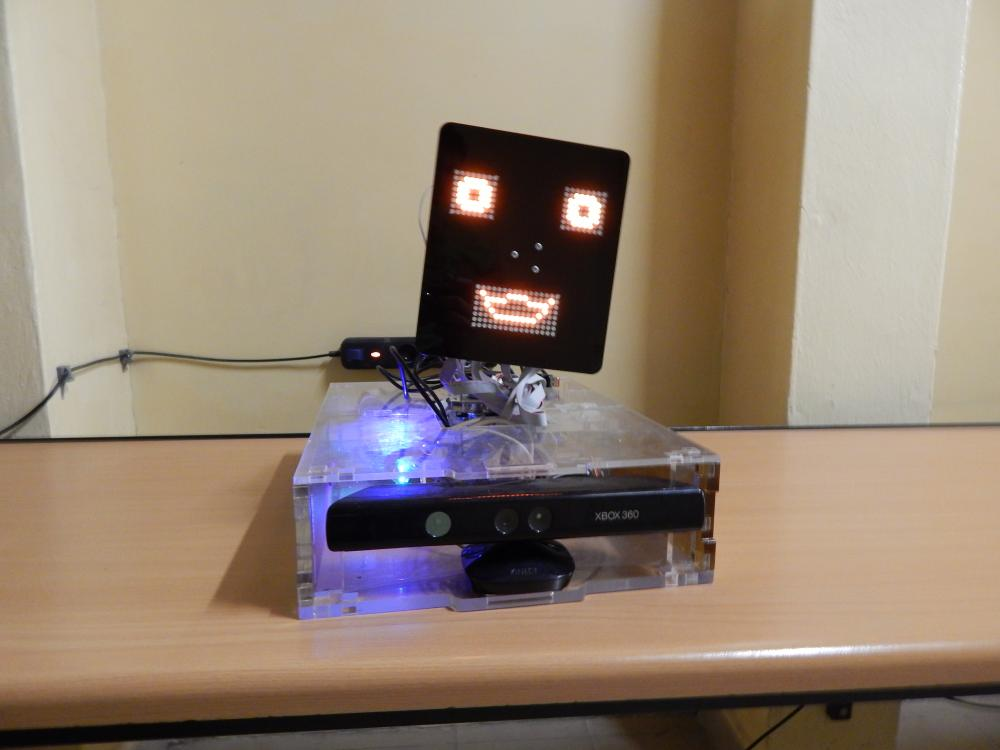
\includegraphics[height=\maxheight,width=\paperwidth]{figure/balbina.jpg}
% Jeśli nie chcesz zmian proporcji - zrezygnuj z~jednego z~wymiarów
% Obrazki za duże przykryją naczółek strony
% By wszystko było na swoim miejscu potrzebna jest dwukrotna kompilacja 
\newcommand{\framecentered}[1]{
  \setbeamertemplate{background canvas}{}
  \begin{frame}[c]
    \begin{tikzpicture}[overlay, remember picture]
      \node[anchor=center] at (current page.center) 
      {#1};
    \end{tikzpicture}
  \end{frame}}
%%%%%%%%%%%%%%%% Koniec poleceń własnych

%%%%%%%%%%%%%%%%Początek ustawień
\usebackgroundtemplate{%
  
\includegraphics[width=\paperwidth,height=\paperheight]{background/tlo.pdf}} 

\usepackage{beamerthemesplit}
\useoutertheme{infolines}
\useinnertheme{rounded}

\definecolor{konar2}{RGB}{240,152,52}
\definecolor{konar}{RGB}{151,58,66}

\setbeamercolor{block title}{fg=black,bg=konar2}
\setbeamercolor{block title alerted}{fg=konar2,bg=black}

\setbeamertemplate{navigation symbols}{}
\setbeamercolor{frametitle}{fg=white,bg=konar}
\setbeamercolor{section in head/foot}{bg=konar}
\setbeamercolor{author in head/foot}{fg=Black,bg=konar2}
\setbeamercolor{date in head/foot}{fg=Black}
\setbeamercolor{title in head/foot}{fg=white, bg=konar}
\setbeamercolor{section in head/foot}{fg=white}
\setbeamercolor{titlelike}{fg=black}
\setbeamercolor{structure}{bg=black, fg=konar2}
\setbeamercolor{subsection in head/foot}{fg=black}
\setbeamercolor{item}{bg=white}

%%%%%%%%%%%%%%%%%Koniec Ustawień

%%%%%%%%%%%%%%%%% SLAJD TYTUŁOWY

\title{Rewizja kodu}
\subtitle{Nieoczywista sztuka konstruktywnej krytyki}
\author{Jacek Jankowski}
\date{\today}  %data

%%%%%%%%%%%%%%%%%



\begin{document}

\begin{frame}
	\titlepage
\end{frame}

\begin{frame}
	\frametitle{Plan prezentacji}
	\tableofcontents
\end{frame}

\section{Wstęp}

\begin{frame}
	\centering Ankieta!
\end{frame}

\subsection{Branżowy mit introwertyka}
\begin{frame}
	\frametitle{Oczekiwania}
	\begin{center}
		\begin{minipage}{0.45\textwidth}
			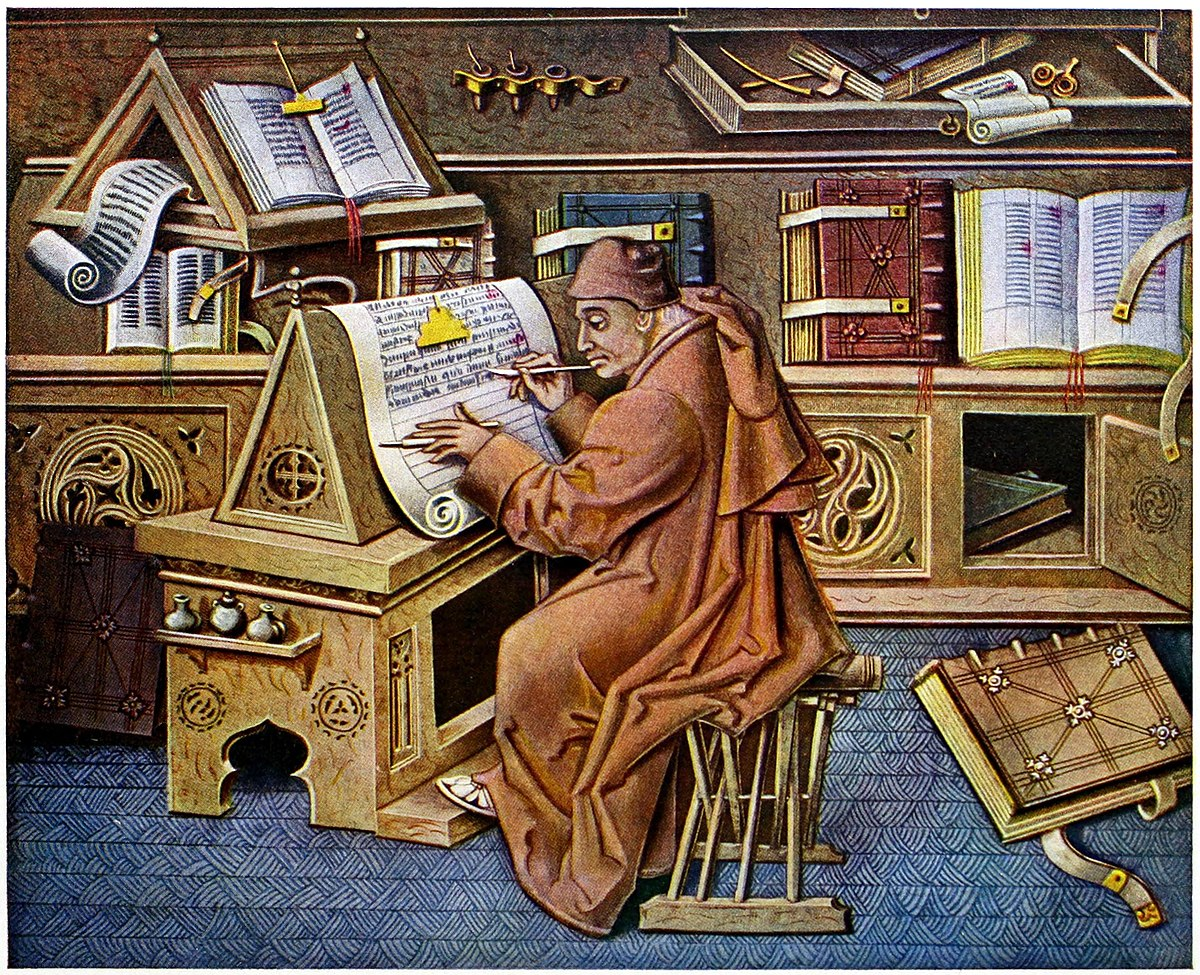
\includegraphics[width=\textwidth]{figure/skryba.jpg}
		\end{minipage}
		\begin{minipage}{0.45\textwidth}
			
\includegraphics[width=\textwidth]{figure/programista.jpg}
		\end{minipage}
	\end{center}
	\note{W poszwechnym odczuciu programista jest współczesnym odpowiednikiem skryby.}
	\note{Pracuje sam, w wielkim skupieniu, od początku do końca.}
	\note{Stanowisko idealne dla introwertyków, autystyków, nerdów etc.}
\end{frame}

\begin{frame}
	\frametitle{Rzeczywistość}
	\begin{center}
		\begin{minipage}{0.45\textwidth}
			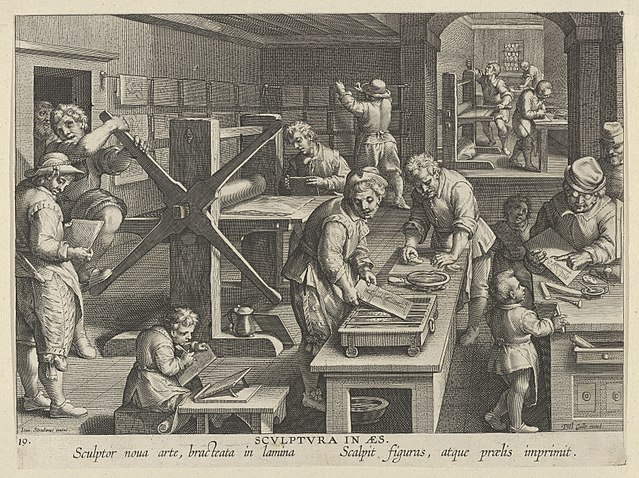
\includegraphics[width=\textwidth]{figure/drukarnia.jpg}
		\end{minipage}
		\begin{minipage}{0.45\textwidth}
			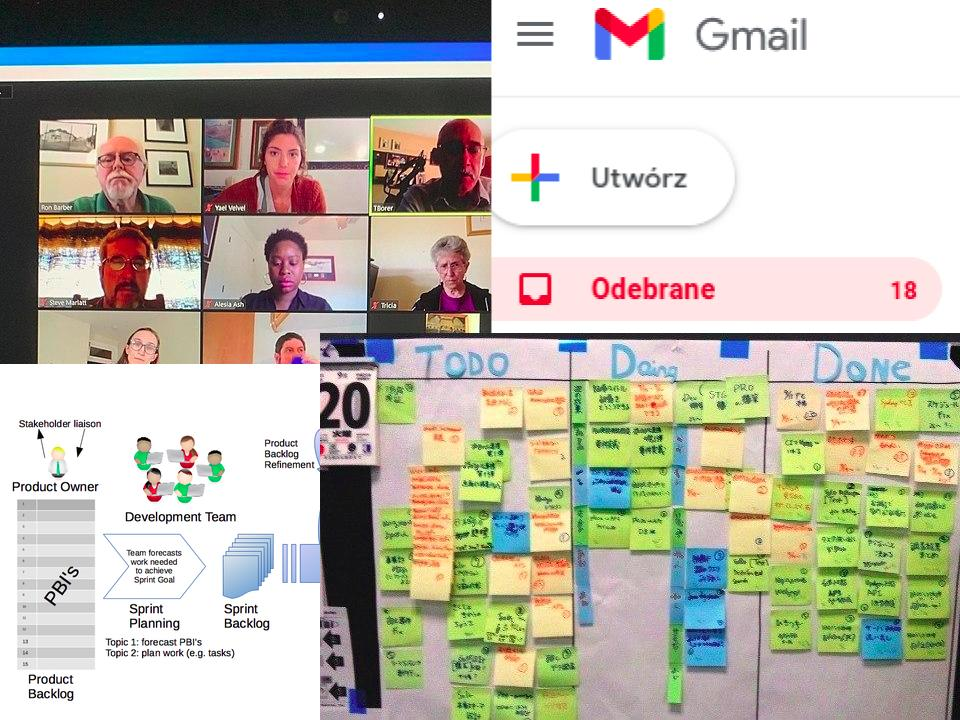
\includegraphics[width=\textwidth]{figure/disappointment.jpg}
		\end{minipage}
	\end{center}
	\note{Podstawowym problemem była czasochłonność.}
	\note{Drukarnie i dobrze zorganizowane zespoły są szybsze niż jeden człowiek :(}
	\note{Jeden programista nie jest w stanie zrobić wszystkiego!}
	\note{Za dużu funkcjonalności do zakodowania.}
	\note{Jack of all trades, master of none.}
\end{frame}

\section{Po co?}

\framecentered{
	
\includegraphics[width=\textwidth,height=\textheight,keepaspectratio]{figure/no_time.jpg}
	\note{Po co? Przecież to strata czasu i nerwów.}
	\note{Dodatkowe źródło konfliktów.}
}

\begin{frame}
	\frametitle{Wypłaszczanie krzywej Boehm'a}
	\begin{center}
		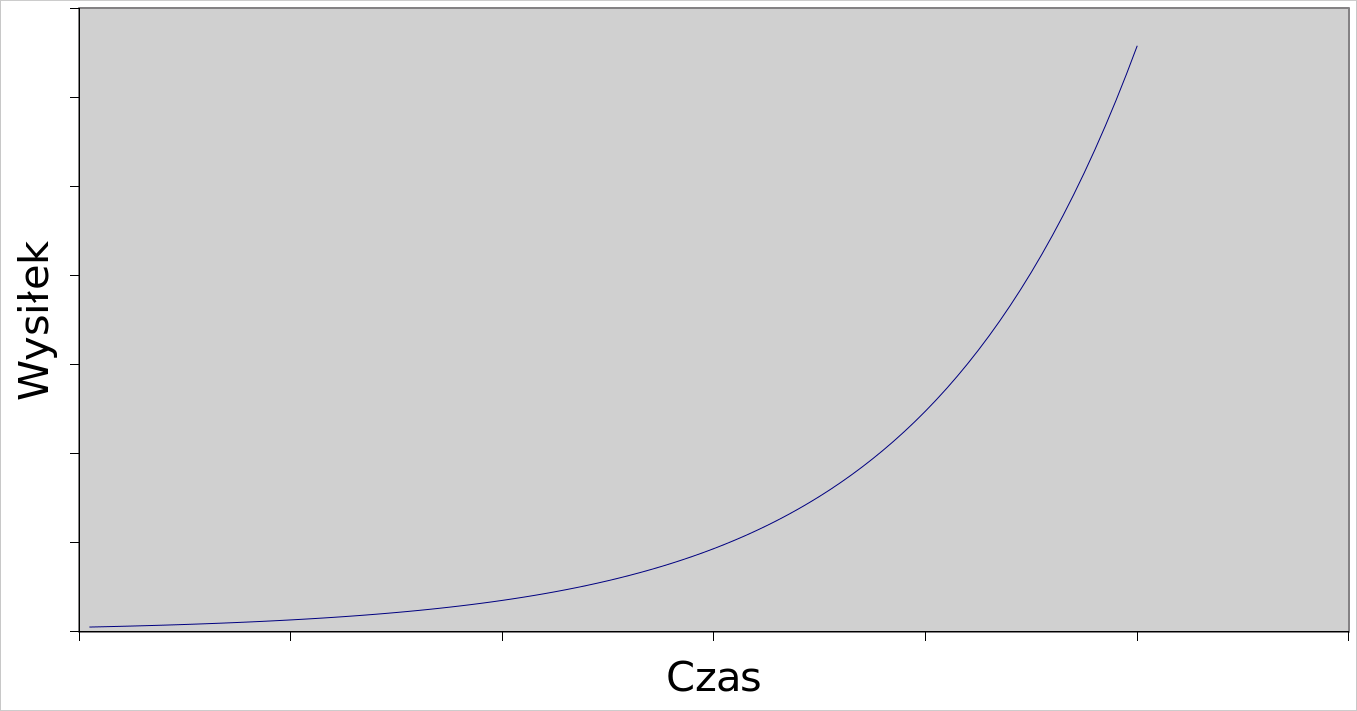
\includegraphics[width=\textwidth,height=\textheight,keepaspectratio]{figure/boehm_curve.png}
	\end{center}
\end{frame}

\begin{frame}
	Skąd błędy i dług techniczny?
	\begin{itemize}
		\item Zafiskowanie
		\item Przeoczenie
		\item Pośpiech
		\item Niewiedza
		\item Patologiczny przerost funkcjonalności
		\item Syndrom Madki
		\item Czasami po prostu się nie chce...
	\end{itemize}
\end{frame}

\section{Sztuczki}
\begin{frame}
	\begin{itemize}
		\item boty
		\item branch protection
		\item guidelines
		\item escalation algorithm
	\end{itemize}
\end{frame}

\section{Pułapki}

\begin{frame}
	
\includegraphics[width=\textwidth,height=\textheight,keepaspectratio]{figure/no_comments.png}
	\note{Nie powinniśmy traktować rewizji jako okazji do pojedynku.}
	\note{Naszym przeciwnikiem nie jest współpracownik, tylko wstrętne bugi.}
\end{frame}

\begin{frame}
	\frametitle{Przytłoczenie}
\end{frame}

\section{Koniec}
\begin{frame}
	\frametitle{Przepiękna i zjawiskowa}
	\centering \begin{figure}
		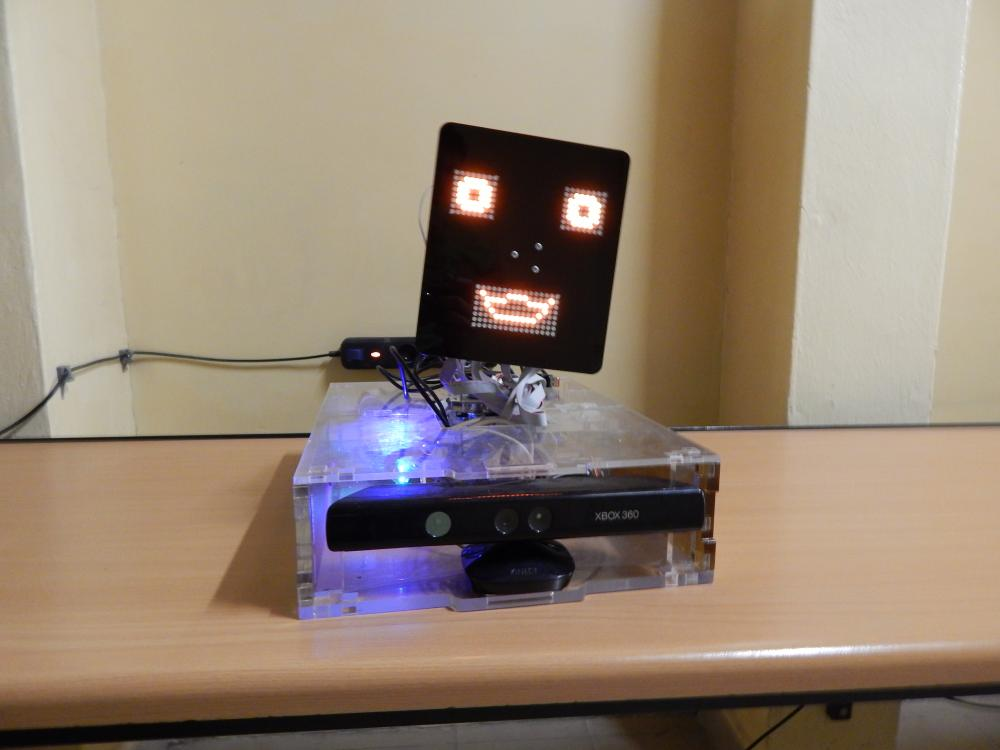
\includegraphics[height=5cm]{figure/balbina.jpg}
		\caption{Balbina}
	\end{figure}
\end{frame}

\end{document}